\documentclass[]{article}
\usepackage[UTF8]{ctex}
\usepackage{amsmath}
\usepackage{graphicx}
\usepackage{ntheorem} %为了proof没有编号

\usepackage{mathrsfs} %为了有花体字

\newtheorem{theorem}{定理}
\newtheorem{definition}{定义}
\newtheorem{corollary}{推论}
\newtheorem*{proof}{证明}

%控制页边距,7in:表示页面宽度最大值  10in:表示页面高度最大值
\usepackage[a4paper, total={7in, 10in}]{geometry}

%opening
\title{与分布式计算相关的几个复杂性问题}
\author{姚期智\\
	斯坦福大学,施乐实验室\\
{\small  翻译:李晓峰(cy\_lxf@163.com)}\\
{\small  译文来自于经典文献翻译项目https://gitee.com/uisu/InfSecClaT}\\
{\small 北京联合大学智慧城市学院}
}

\begin{document}
	
	\maketitle
	
	\begin{abstract}
		此文是对姚期智老师Some Complexity Questions Related to Distributive Computing文章的翻译。
	\end{abstract}
	
	\section{引言}
	设$M=\{0,1,2,\ldots,m-1\},N=\{0,1,2,\dots,n-1\}$,$f:M\times N \rightarrow \{0,1\}$是一个布尔值函数,我们看一下下面这个问题,以及其他相关的问题。\par
	设$i\in M,j\in N$分别是$P_1$和$P_2$知道的两个秘密数,也就是i只有$P_1$知道,j只有$P_2$知道,现在$P_1,P_2$要合作计算$f(i,j)$,她俩依据某个算法分别向对方发送信息,每次只发送1比特信息,我们感兴趣的数值是:在所有算法中,最小的比特数是多少,这个值度量了计算所需的交换信息。\par
	例如:对于$f(i,j)=(i+j)\pmod{2}$,$P_1$只需发1比特的信息(传输i是否为奇数)给$P_2$,$P_2$就可以计算$f(i,j)$,在这个计算中,这个显然是个最好的解决办法(译者注:因为只用传输一个比特就能进行计算.)。\par
	上面的问题是Abelson[1]在分布式计算信息传输模型的变种,在Abelson的模型中,$P_1,P_2$计算一个“smooth”的实数值函数$f(x_1,x_2,\ldots,x_s;y_1,y_2,\ldots,y_t)$,$P_1$知道$x_1,x_2,\ldots,x_s$,$P_2$知道$y_1,y_2,\ldots,y_t$。假定$P_1$和$P_2$可以相互发送平滑函数值,Abelson获得了为了计算f需要交换的下限,我们的模型对应这样一种情况,f是布尔函数,x和y是布尔变量$(m=2^s,n=2^t)$,交换的值是比特。与Abelson的模型特点相比,本文的框架解决的实质上是组合计算。
	
	\section{确定性模型}
	考虑在$P_1,P_2$间控制比特交换的算法是确定性算法,$P_1$知道i,$P_2$知道j.计算过程是这样的:
	\begin{itemize}
		\item $P_1$发送$a_1\in\{0,1\}$给$P_2$。
		\item $P_2$收到$a_1$后,发送$b_1$给$P_1$。
		\item $P_1$收到$b_1$后,发送$a_2$给$P_2$。
		\item ......
	\end{itemize}
	\par
    $a_k$或$b_k$的选择依赖于截止选择之时通信的所有比特。准确地描述,算法A描述这样一组布尔函数\\
    $\{h_k(i;u_1,u_2,\ldots,u_{k-1}),$ $l_k(j;v_1,v_2,\ldots,v_k) | k=1,2,\ldots \}$,$a_k=h_k(i;b_1,b_2,\ldots,b_{k-1})$,$b_k=l_k(j;a_1,a_2,\ldots,a_k)$,当$P_1$或$P_2$有足够的信息确定$f(i,j)$是,计算停止,然后发送“halt”字符给另一方。\par
    代价$\alpha(A)$定义为对于任意i和j,算法A所需交换的最大比特数。\par
    $f$的双向复杂性定义为:\footnote{译者注:其含义是所有算法中的最小代价。}
    \[C(f:1\leftrightarrow 2)=min\{\alpha(A) | A\ computes\ f\}\]
    \par
    为了研究C的大小,我们用一种更方便的方法来看计算这个过程。不难看出,以上的算法我们可以这样来描述,我们用一个例子来说明。\par
    设f是一个函数,用图\ref{Fig1}来定义,计算$f$的算法A如图\ref{Fig2}中的决策树所示。\par
    \begin{figure}[htbp]
    	\centering
    	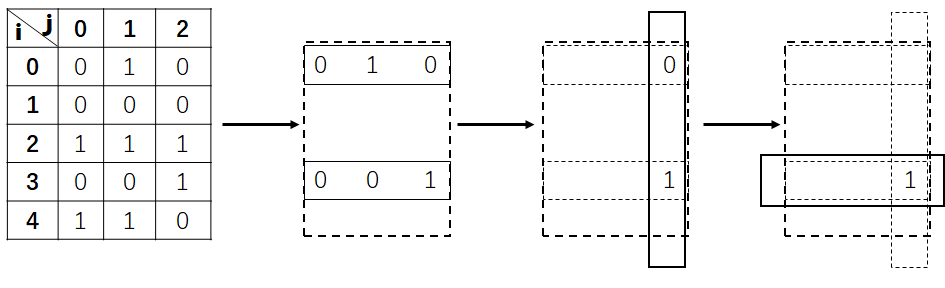
\includegraphics[width=0.7\textwidth]{Fig1.png}
    	\caption{函数f,算法查找$f(3,2)$的执行步骤}
    	\label{Fig1}
    \end{figure}

	\begin{figure}[htbp]
		\centering
		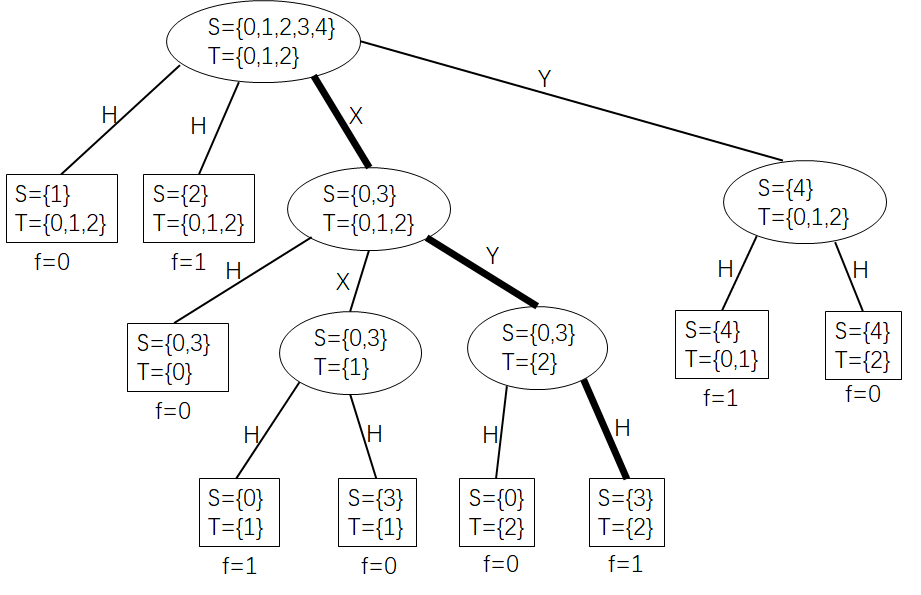
\includegraphics[width=0.7\textwidth]{Fig2.png}
		\caption{一个计算函数f的算法,对于输入i=3,j=2,交换的信号序列为XYH}
		\label{Fig2}
	\end{figure}

	图\ref{Fig2}中中间节点最多有4个子节点(两个叶子,两个子节点),引向叶子的分支标为H(Halt),引向子节点的分支标为X或Y(我们用X,Y代表0,1,以免与函数值混淆)。从根开始,$P_1,P_2$交替移动,所以1,3,5,$\ldots$步的信号是$P_1$发送,2,4,6,$\ldots$步的信号是$P_2$发送,每个叶子都赋予一个比特,是f(j,j)的值,下面我们来描述在一个内部节点上如何选择分支。\par
	
	每一个节点v关联一个矩阵$S(v)\times T(v)\subseteq M\times N$,根节点r关联的矩阵为$S(r)\times T(r)= M\times N$。\par
	对于一个在奇数层(根节点的层数为1)的内部节点v,其有子节点$v_1,\ldots,v_l(l\leq 4)$,我们有:
	\begin{itemize}
		\item 如果$1\leq k \leq l $,那么$T(v)=T(v_k)$;\footnote{译者注:奇数层的子节点,其T集合同父节点。}
		\item $\{S(v_k) | 1\leq k \leq l\}$,形成$S(v)$的一个不相交的分割;
	\end{itemize}
	\par
	
	对于偶数层,$S$和$T$的情形调转,也就是:
	\begin{itemize}
		\item 如果$1\leq k \leq l $,那么$S(v)=S(v_k)$;
		\item $T(v_k) | 1\leq k \leq l$,形成$T(v)$的一个不相交的分割;
	\end{itemize}
	\par
	
	当$P_1$从一个奇数层节点$v$移动时,他移到子节点$v_k,i\in S(v_k)$\footnote{译者注:例如在图\ref{Fig2}中的情况来说,$P_1$的秘密数是$i=3$,那么其将会移动到包含$S$中包含3的节点上去,下面说“$P_2$情况也相同”,意思是在偶数层$P_2$发送比特,$P_2$的秘密数是$j=2$,那么其会移动到$T$中包含2的节点上去。}。$P_2$情况也相同。节点$v$是叶子节点,当且仅当在块$S(v)\times T(v)$中,$f$是常数。对于算法A,我们有$\alpha (A)=height(A)-1$。\footnote{译者注:节点深度(depth)是祖先个数,不包括节点本身,等价为节点到根有多少条边。节点高度(height)是其孩子节点中最大高度加1,叶子节点高度为0,树的高度是树根节点的高度。}
	\par
	归纳$mn$个函数值的计算情况,任何一种算法都可以表示成上述形式,我们将证明一些结论。
	\par
	
	\begin{definition}\footnotemark
		设$f$是一个在$M\times N$上的布尔值函数,$S\subseteq M,T\subseteq N$,如果$f$在$S\times T$上是个常数,我们将笛卡尔积$S\times T\ $称为一个$f$单调矩形($f$-monochromatic rectangle )。函数$f$的$k$分解($k$-decomposition )是由$k$个不相交的f单调矩形组成的集合(family)$\zeta=\{S_1\times T_1,S_2\times T_2,\ldots,S_k\times T_k\}$,这$k$个不相交的$f$单调矩形是$M\times N$的一个分割。设$d(f)$是存在的所有$f$的$k$分解的最小$k$值。
	\end{definition}
	\footnotetext{
		译者注:我们以图\ref{Fig1}中函数为例,看看上述概念的含义,$M=\{0,1,2,3,4\},N=\{0,1,2\}$,我们可以看到$\{1\}\times \{0,1,2\}$,$\{2\}\times \{0,1,2\}$,$\{3\}\times \{0,1\}$,$\{0,1,3\}\times \{0\}$,$\{4\}\times \{2\}$均是$f$的单调矩形。\\
		函数$f$的8分解:$\{0\}\times \{0,2\}$,$\{0\}\times \{1\}$,
		$\{1\}\times \{0,1,2\}$,
		$\{2\}\times \{0,,1,2\}$,
		$\{3\}\times \{0,1\}$,$\{3\}\times \{2\}$,
		$\{4\}\times \{0,1\}$,$\{4\}\times \{2\}$\\
		函数$f$的6分解:$\{0,1,3\}\times \{0\}$,$\{2,4\}\times \{0\}$,
		$\{0,2,4\}\times \{1\}$,$\{1,3\}\times \{1\}$,
		$\{0,1,4\}\times \{2\}$,$\{2,3\}\times \{2\}$
		\\
	}
	
	
	\begin{theorem}\label{th1}\footnotemark
		 $C(f;1\leftrightarrow 2) \geq \log_2{d(f) -2} .$
	\end{theorem}
	\footnotetext{
		译者注:我么先从直观上看看这个定理,我们已经知道函数的最小分解数,如果用这个最小分解构造一个判定树,要看看其有多少条分支,把第一层我们可以有两个页节点,所以$\xi = d(f)-2$,剩下的我们就是用2进制编码,每个叶节点一个唯一编码$log_2 \xi$,显然这个应该是下限。
	}
	
	
	\begin{corollary}\label{coro1}
		设$\mathscr{F}_n$是所有在$N\times N$上的布尔函数,随机取一个$f\in \mathscr{F}_n$,$f$满足$C(f;1\leftrightarrow 2)\geq \log_2 n -4$的概率是$1-O(2^{-\frac{n^2}{2}})$.
	\end{corollary}
	

	\begin{proof}
		设A是选择计算$f$的算法,使用前面的树来描述,每一个内部节点最多有两个叶子节点,因此:\par
		\begin{equation}\label{eq:1}
			\begin{aligned}
			d(f) & \leq number\ of\ leaves\footnotemark[8] \\
			& \leq 2 \times I(f)\footnotemark[9] ,
			\end{aligned}
		\end{equation}
		\footnotetext[8]{因为不同的叶子,其函数取值可能一样,所以那个最小分解数一定小于等于叶子数。}
		\footnotetext[9]{每个内部节点最多有个两个叶子节点,所以叶子节点数应该小于2倍的内部节点。}
		\par
		此处$I(f)$是f的内部节点数,内部节点构成的这棵树,高度为$\alpha(A)$,分支最多为2,我们有:\footnote{译者注:因为在构造这棵树时,我们规定最多四个节点,最多两个叶子,最多两内部节点,图\ref{Fig2}有5个内部节点(根也算),$\dfrac{I(f)+1}{2}=3,\alpha(A)=3$}
		\par
		\begin{equation}\label{eq:2}
			\dfrac{(I(f)+1)}{2} \leq 2^{\alpha(A)}.
		\end{equation}
		\par
		根据公式\ref{eq:1}和公式\ref{eq:2},我们可得:\par
		\begin{equation}\nonumber
			2^{\alpha(A)}\geq \dfrac{d(f)}{4}
		\end{equation}
		\par
		这意味着:\footnote{译者注:对于上式两边取$\log_2$,得$\alpha(A)\geq \log_2 d(f) -2$,复杂度时$\alpha(A)$最小值,所以有$C(f;1\leftrightarrow 2)\geq \log_2 d(f) -2$}
		\par
		\begin{equation}\nonumber
		    C(f;1\leftrightarrow 2)\geq \log_2 d(f) -2.
		\end{equation}
		\par
		定理\ref{th1}得证。$\spadesuit$
	\end{proof}
	\par
	\begin{proof}
		(推论\ref{coro1}). $S\subseteq N,T\subseteq N$,$S,N$可以是空集,那么形如$S\times T$的集合最多有$2^{2n}$个,满足$d(f)\leq k$的函数$f\subseteq \mathbf{F}_n$最多有$2^{2kn}$个,现在,在$\mathbf{F}_n$中最多有$2^{n^2}$个不同的函数,满足$d(f)>\frac{n}{4}$(因此$C(f;1\leftrightarrow 2)> \log_2 n -4$)的函数至少为:
		\[(2^{n^2}-2^{2nn/4})/2^{n^2} = 1-O(2^{-n^2/2})\]
		推论得证。$\spadesuit$
	\end{proof}
	\par
	因为$ C(f;1\leftrightarrow 2)\leq 2 \left[  \log_2 n \right] $($P_1$可以简单发送表示i的二进制给$P_2$),上面的推论确定了所有布尔函数复杂度两倍。\par
	
	下面我们给出一些特别的函数,它的复杂度$ C(f;1\leftrightarrow 2)$是$\log n$,这个可以根据定理\ref{th1}获得(证明略)。\par
	
	\textbf{例子1:}识别函数(identification function):$f(i,j)=\delta_{ij}$,$i,j\in \{0,1,\ldots,n-1\}$.\par
	
	\textbf{例子2:}互素测试函数(relatively-prime testing fimction):$f(i,j)=1$,当且仅当i和j互素,$i,j\in \{0,1,\ldots,n-1\}$.\par
	
	\textbf{例子3:}排序函数( ordering function):$f(i,j)=1$,当且仅当$0\leq i \leq j < n$.\par
	
	\textbf{例子4:}集合相交函数(set-intersection function):$f(i,j)=1$,当且仅存在某个k,i和j的第k个比特均为1,$i,j\in \{0,1,\ldots,n-1\}$。\par
	
	做为$k$的函数,定理给出的边界有多好?下面的定理可以回答这个问题(高达一个常数因子),如果$f$有一个平的(planar)$d(f)$-分解。\par
	
	\begin{definition}
		$f$的一个$k$分解,$\zeta=\{S_1\times T_1,S_2\times T_2,\ldots,S_k\times T_k \}$,如果每一个$S_l$(和$T_l$)由一个连续的整数块组成,那么我们称此k分解是平的(planar)。
	\end{definition}

	\begin{theorem}
		如果$f$有一个平的$k$-分解($k\geq 1$),那么
		\[C(f;1\leftrightarrow 2)\leq \dfrac{2\log_2 k}{\log_2(4/3)}  +6 \].
	\end{theorem}
	
	\begin{proof}
		显然$C(f;1\leftrightarrow 2)\leq k$,那么对于$k\leq 4$,定理成立。下面我们用归纳法证明对所有的$k\geq 5$,
		\begin{equation}\label{equa3}
			C(f;1\leftrightarrow 2)\leq \dfrac{2\log_2 (k-4)}{\log_2(4/3)}  +6
		\end{equation}
		这个不等式对于$k=5,6$显然成立,现在假设$k\geq 7$.\par
		
		我们会证明的,对于某些函数$f_1,f_2$,每一个都有一个平的$([3k/4]+1)$-分解,
		\begin{equation}\label{equa4}
			C(f;1\leftrightarrow 2)\leq 2+max\{C(f_a;1\leftrightarrow 2) | a=1,2\}
		\end{equation}
		利用这个归纳假设,可得
		\[C(f;1\leftrightarrow 2) \leq 2+ \dfrac{2(\log_2([3k/4]+1-4))}{\log_2(4/3)} +6 \leq \dfrac{2(\log_2(k-4))}{\log_2(4/3)} +6\]
		至此完成归纳。\par
		下面需要证明假设\ref{equa4},我们分为两种情况。\par
		情况A:存在$s\in M$,那么有$h\geq [k/2]$个不同的$S_l\times T_l,i\in S_l$。不失一般性,我们可以假定他们是$S_1\times T_1,S_2\times T_2,\ldots,S_h\times T_h$,$T_1,T_2,\ldots,T_h$是连续的间隔覆盖集合$N=\{0,1,\ldots,n-1\}$。设$N_1=T_1\cup T_2 \cup \ldots \cup T_{[h/2]}$,$N_2=N-N_1$,我们易知,对于$j\in \{1,2,\ldots,k\}$,每个$M\times N_a(a=1,2)$最多相交$k-[h/2]\leq (3k/4)+1$组$S_l \times T_l$.因此,f对$M\times N_a$的限制,每个$f_a(a=1,2)$有一个平的$([3k/4]+1)$-分解。因为$P_2$可以通过1比特与$P_1$通信,告诉$P_1$,$P_2$拥有的变量j是否在$N_1$或$N_2$,我们得到公式\ref{equa4}.
		\par
		情况B:假定情况A中的条件不满足,设$s\in S$是最小的s,所以至少有$k/4$个$S_l\times T_l \subseteq M_1\times N$,$M_1=\{0,1,\ldots,s\}$,用$M_2$表示$M-M_1$,每个$S_l$是一个区间(interval),任何$S_l\times T_l$与$M_1\times N$的交集一定满足$s\in S_l$或者$S_l \times T_l\subseteq (M_1-\{s\})\times N$,这意味着最多$[k/2]+k/4 \leq 3k/4 +1 $个集合$S_l\times T_l$与$M_1\times N$相交,所以,与$M_a\times N$相交的$S_l\times T_l$集合最多有$[3k/4 + 1]$个,对于每个$f$到$M_a\times N$的限制$f_a$,有一个平的$[3k/4]+1$-分解,$P_1$只需发送给$P_2$1比特就足够表示变量$P_1$拥有的变量$i$是否在$M_1$,公式\ref{equa4}成立。
		\par
		至此完成定理证明。$\spadesuit$
	\end{proof}
	\par
	
	对于一般的非平分解,我们有如下定理。\par
	\begin{theorem}\label{theo3}
		存在常数$\lambda >0$,那么,对于所有$f$,我们有:
		\[C(f;1\leftrightarrow 2)\leq \lambda \sqrt{d(f)\log_2 d(f)}\]
	\end{theorem}
	\begin{proof}
		(证明梗概)设$k=d(f)$,我们对于归纳$k$证明定理。\par
		对于每个$s\in M$,设$pat_s = \{l | s\in S_l\}$,这里存在$s$,使$|pat_s| \geq 2\sqrt{k/log_2 K}$,或者不同的$pat_s$总共不超过
		\begin{equation}\nonumber
		 \left(
			\begin{array}{c}
			    k \\
			    \left[ 2 \sqrt{k/log_2 k}\right] 
			\end{array}
		\right) \leq e^{\lambda_1 \sqrt{k\log_2 k}}
		\end{equation}
		\\
		此处$\lambda_1 >0$是一个常数。在前一种情况下,通过一个类似于上一个定理的论证,我们可以证明存在$f_a(a=1,2)$,且$f_a\leq k-\left[ \sqrt{k/log_2 k} \right] $,我们可得:
		\begin{equation}\label{equa5}
			C(f;1\leftrightarrow 2)\leq 2+ max\{C(f_a;1\leftrightarrow 2)|a=1,2\}
		\end{equation}
		\\
		在后一种情况,$P_1$给$P_2$发送$O(\lambda_1 \sqrt{k\log_2 K})$比特,可以使$P_2$立即确定$f$的值。在这两种情况下都可以执行归纳。
		\par
		定理\ref{theo3}得证。$\spadesuit$
	\end{proof}
	
	
	

	\section{概率模型}
	最近算法设计中一个有趣的创新是加入了随机移动和允许c概率的错误(参见Rabin[2]),如果给每个参与者$P_i$一个随机数发生器,它们能用更少的信息交换来确定f的值吗?在此我们讨论两种模型。
	
	\subsection{单向概率通信}
	为了确定$f(i,j)$,参与者$P_i$给$P_2$随机发一个字符串,基于这个字符串$P_2$随机决定$f(i,j)$的值,错误的概率小于等于$\epsilon$。这里有几种不同的方法来定义复杂度。为简单起见,设所有被传输的字符串长度一样。$f$的单向概率复杂度(l-way prbabilistic complexity)$C_{\epsilon}'(f;1\rightarrow 2)=\left[ \log_2 k\right] $,此处$k$是使以下不等式组满足的最小整数,下式中$\vec{p_i}=(p_{i_1},p_{i_2},\ldots,p_{i_k}),1\leq i \leq m,\vec{q_j}=(q_{j_1},q_{j_2},\ldots,q_{j_k}),1\leq j \leq n$.\\
	\begin{equation}\label{equa6}
		\left\lbrace 
		\begin{array}{l}
			\sum_{l}^{} {p_{i_l}} =1;\ for\ all \ i,j\\
			p_{i_l}\geq 0;\ 1\geq q_{i_l}\geq 0\ for \ all i,j,e\\
			\vec{p_i}\vec{q_j}\geq 1-\epsilon ; \ if\ f(i,j)=1,\\
			\vec{p_i}\vec{q_j}<\epsilon; \ if\ f(i,j)=0
		\end{array}
		\right. 
	\end{equation}
	\par
	\textit{备注:}把$(f(i,j))$看做一个0-1矩阵,并将这个矩阵不同的行和列的数量分别记为$nrow(f),lcol(f)$,对这种确定的情况单向复杂度( 1-way complexity)我们很容易确定是$[\log_2(nrow(f))]$。
	\par
	在第二部分定义的标识函数(identification function),对于这个特例的,Rabin和Yao[3]进行了研究,是$loglog n$。对于一个随机的函数,下面的结果确定其$C'_\epsilon$,然而一般来讲,对于明确的函数确定$C'_\epsilon$看起来是困难的。
	
	\begin{theorem}\label{theo4}
		设$\epsilon$是在$0<\epsilon < 1/2$范围内容的一个固定的数,记$\mathscr{F}_n$是所有$N\times N$上的布尔函数集合,那么随机选取一个函数$f\in \mathscr{F}$,其以概率$1-O(2^{-\frac{n^2}{2}})$满足
		\[[\log_2 n] \geq C'_\epsilon (f;1 \rightarrow 2) \geq [\log_2 n]-\log_2 \log_2 n -2 \]
	\end{theorem}
	
	\begin{proof}
		第一个不等式对所有$f$显然成立,所以我们只看第二个不等式。\par
		$\mathscr{F}_{n,k}\subseteq \mathscr{F}_n$,$\mathscr{F}_{n,k}$是所有向量$\vec{p_i},\vec{q_j}$的k分量(k-component)满足不等式组\ref{equa6}的函数$f$集合,对于每个$f\in \mathscr{F}$,我们选择一个解决方案(solution),并且定义一个(2kn)-元组((2kn)-tuple)
		\[\gamma(f) = (\lceil 4 p_{ij}k/(1-2\epsilon)  \rceil , \lceil4q_{ij}k/(1-2\epsilon) \rceil \ |\ 1\leq i\leq n,1 \leq j \leq k )\]
		我们称$\gamma(f)$为$f$的一个代表(representative),很明显,这里代表数最多有:
		\[(1+\lceil 4k/(1-2\epsilon)\rceil )^{2kn} =exp(2kn \ln k + O(1))\]
		\par
		现在我们断言,在$\mathscr{F}_{n,k}$中,没有两个不同的函数$f$和$f'$,他们有相同的代表。否则,我们设$\vec{p_i},\vec{q_j}$和$\vec{p'_i},\vec{q'_j}$,分别于$f$和$f'$关联,选择$s,t$,$f(s,t)\neq f'(s,t)$,根据公式\ref{equa6},我们有:\\
		\begin{equation}\label{equa7}
			| \vec{p_s}\vec{q_t} - \vec{p'_s}\vec{q'_t} | \geq 1-2\epsilon
		\end{equation}
		另一方面,当$f$和$f'$有相同的代表时,我们有
		\begin{equation}\nonumber
			\begin{aligned}
			    \left| \vec{p_s} \vec{q_t} - \vec{p'_s} \vec{q'_t} \right|  & \leq \sum_{l} p_{sl}|q_{tl}-q'_{tl}|+ q_{tl}|p_{sl}-p'_{sl}|\\
		                                                       & \leq 2k\dfrac{1-2\epsilon}{4k}  \\
		                                                       & < 1-2\epsilon
			\end{aligned}
		\end{equation}
		与公式\ref{equa7}想矛盾,断言得证。\par
		根据上面的讨论,我们有
		\[\dfrac{|\mathscr{F}_{n,k}|}{|\mathscr{F}_n|} \leq \dfrac{exp(2kn\ln k +O(1))}{2^{n^2}}\]
	
	    取$k=n/(4\ln n)$,我们得到结论,$C'_\epsilon (f;1 \rightarrow 2) \geq [\log_2 n]-\log_2 \log_2 n -2$的概率最大是$O(2^{-n^2/2})$。
		\par
		定理\ref{theo4}得证。$\spadesuit$
	\end{proof}
	
	\subsection{双向概率通信}
	在第二部分基本双向模型中,允许在两个参与者中概率移动,设$\epsilon(0<\epsilon<1/2)$是允许的错误概率,定义是在算法A下,最坏输入情况下,期望传输的比特数为$\alpha'(A)$,设$C'_\epsilon(f;1\leftrightarrow 2)=inf\{\alpha'(A)\ |\ A \text{算法最大错误概率}\epsilon\}$。下面的结果给出了概率算法的能力限制,例如,其表示标识函数双向概率复杂度也是$\log \log n$阶。\par
	
	\begin{theorem}\label{theo5}
		设$\epsilon(0<\epsilon<1/2)$是个确定数,那么存在一个常数$\lambda'>0$,对于任意$f$,
		\[C'_\epsilon (f;1\leftrightarrow 2) \geq \lambda'(\log_2 \log_2(nrow(f))+ \log_2\log_2 (ncol(f)) )\]
    \end{theorem}
	
	\begin{proof}
		因为他的复杂性,我们此处略掉证明。$\spadesuit$
	\end{proof}

	\section{总结}
	本文我们研究当两方合作计算一个布尔函数时所需交换的信息量,确定性单向模型在数学上已经讨论的很清楚了,下面我们将给出理解其他三个模型的建议,提出几个公开问题。\par
	
	\textit{A.确定性双向复杂度(The deterministic 2-way complexity).}这个相对来说好理解,几乎$\mathscr{F}_n$中所有的函数其复杂度都约等于$\log n$,对于许多类似函数,复杂度由常数因子决定上限,然而,有一个基本的问题还没有回答,设$a_k = max\{C(f;1\leftrightarrow 2)\ |\ d(f)=k\}$,我们已经知道$c\log k \leq a_k \leq c'\sqrt{k\log k}$,那么$a_k$是什么?\par
	
	\textit{B.概率单向复杂度(The Probabilistic 1-way complexity).}这是未来研究非常有意思的一个主题,我们已经知道$\mathscr{F}_n$中几乎所有函数的复杂度约等于$\log n$,但是没有一个确定的函数其复杂度是这个值,我们猜想第二部分的排序函数(ording function)复杂度大约是$\log n$。\par
	
	\textit{C.概率双向复杂度(The Probabilistic 2-way complexity).}这个不好理解,尽管定理\ref{theo5}给出了下限,但我们甚至不知道$\mathscr{F}_n$中一个随机函数的复杂度,注意,定理\ref{theo5}暗示概率双向通信最多对数级改善确定性单向通信。\par
	
	\textit{D.多于两个参与者.}大多数结果都可以扩展到多与两个参与者的情况,我们指出一种需要特别关注的情况。假设有三个参与者$P_1,P_2,P_3$,合作计算一个函数$f(i,j)$,初始时刻,$P_1$知道i,$P_2$知道j,除了$P_1$和$P_2$之间通信外,假设$P_1,P_2$分别与$P_3$有一个单向概率通信信道(如图\ref{Fig3}),$P_3$以错误概率小于$\epsilon$计算$f(i,j)$,假设$P_3$使用在某个域$M'\times N'$上的布尔值函数$g$,将$f$计算为$g(i',j')$,此处$i',j'$是$P_3$分别从$p_1$和$P_2$接收到的整数,复杂度$C'_\epsilon(f;1\leftarrow 3 \rightarrow 2)$最小是$\log |M'| + \log |N'|$\footnote{译者注:原文是$\log |M'| + \log |M'|$,根据上下文,应该是$\log |M'| + \log |N'|$}在所有可能的$g,M',N'$的选择上。另一个有意思的可选路线是,把$C'_\epsilon(f;1\leftarrow 3 \rightarrow 2)$看作是最小表规模$|M'| |N'|$的$\log$,我们可以利用概率哈希(probabilistic hashing)计算$f(i,j)$,那么,标识函数( identification function)的复杂度是多少?\par
	
	\textit{E.NP-Completeness.}计算复杂度$C(f;1\leftrightarrow 2)$是一个NPC问题吗?
	
		\begin{figure}[htbp]
		\centering
		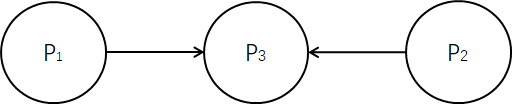
\includegraphics[width=0.7\textwidth]{Fig3.png}
		\caption{第4部分中的$C_{\epsilon}'(f;1\rightarrow 3 \leftarrow 2)$图示}
		\label{Fig3}
	\end{figure}

	
	\vspace{1cm}
	\textbf{参考文献:}\\
	$\left[ 1 \right]$ H. Abelson, Lower Bounds on Information Transfer in Distributed
	Computations, Proc. IEEE 19-th Annual Syrup. on Foundations
	of Computer Science, Ann Arbor, 1978, pp. 151-158.\\
	$\left[ 2 \right]$ M. O. Rabin, Probabilistic Algorithms, in Algorithms and Complexity:
	Recent Results andNew Directions, edited by .L F. Traub, Academic
	Press, 1976, pp. 21-40.\\
	$\left[ 3 \right]$ M. O. Rabin and A. C. Yao, in preparation.
	\par
\end{document}

